% !TeX root = ../thuthesis-example.tex

\chapter{分段对称模式挖掘算法}
第3章介绍了全局对称模式挖掘算法,
然而,真实的对称模式往往是聚合在一条
长时间序列之中的,其中有缺失点、异常点、噪声点等种种干扰,
而且多个对称子序列可能相互重叠在一起,
使得分段对称模式挖掘和结果判断更加困难。
因此,本节设计了一种从长时间序列中挖掘出分段对称模式的算法,
并根据Apache IoTDB的存储和计算方式
对分段对称模式挖掘算法进行了优化。

本章的组织结构如下所示,
4.1节基于分段长度约束$w$,设计了一种计算所有长度
为$w$的时间子序列对称度的算法;4.2节介绍了根据
时间序列数据特征和对称度分布确定分段对称度阈值的算法;
4.3节根据贪心策略和分段对称度阈值挖掘出所有的对称模式;
4.4节分析了基于IoTDB数据库实现分段对称模式挖掘算法
的两种方式,并对比了这两种方式的优劣和适用场景。

\section{分段时间序列对称性度量算法}
要对时序数据进行对称子序列的挖掘,首先要做的就是把时间序列划分成
一段一段的子序列,然后对子序列进行对称度度量。
时间序列断点检测算法是一种经典的时间子序列划分方法\cite{DBLP:conf/igarss/UrbanHZMGBMMFRH21}。
图~\ref{fig:break_detection}展示了时间序列断点检测算法的计算流程。
为了检测时间序列中的关键点,该算法采用直线对整体的时间序列数据
进行拟合,如果时序数据的趋势发生了变化,则用多条直线拟合整条
时序数据。该算法使用单变量线性回归模型拟合每段时间
序列,每处理一个新数据点就重新计算多段拟合误差,利用动态规划算法
全局最大化分段效果。时间序列断点检测算法的好处是可以根据时间序列
的趋势进行关键点的判断,但是,工业时间序列中的分段对称模式多种多样,
除去首尾点之外,模式内部可能也存在关键点,只识别出关键点无法成功
分割出对称模式。此外,时间序列断点检测算法的复杂度高达
$O\left(n^{3}\right)$,甚至超出了对称模式挖掘算法的复杂度,
在实际工业场景中不具备应用价值。
\begin{figure}[t]
  \centering
  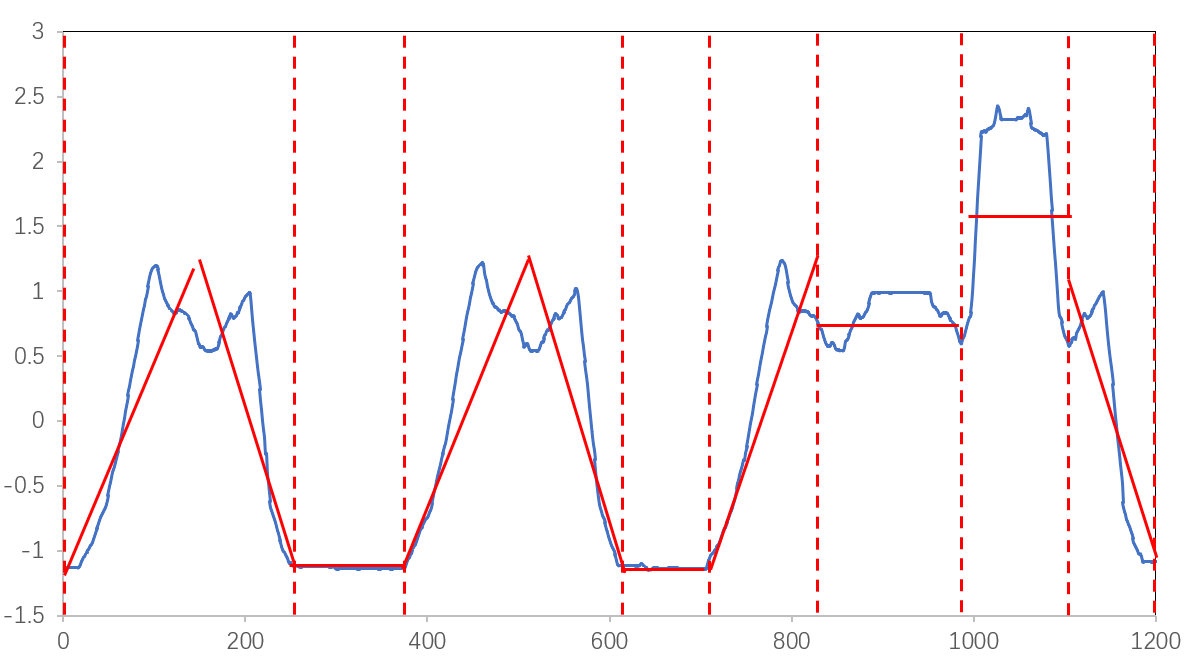
\includegraphics[width=0.66\linewidth]{break_detection.png}
  \caption{时间序列断点检测与直线拟合图}
  \label{fig:break_detection}
\end{figure}

基于此,本文选择基于滑动窗口的时间序列分段算法\cite{DBLP:conf/pkdd/LestiS17}。
滑动窗口源于网络流量控制技术,在时间序列分析领域可以用于在特定窗口大小的子序列上执行对称度计算的
操作。通过维护一个不断向前滑动的窗口,划分出全部的时间序列分段。
图~\ref{fig:sliding_window}展示了使用滑动窗口将时间序列中每个长度为$w$的子序列划分出来的过程。

\begin{figure}[h]
  \centering
  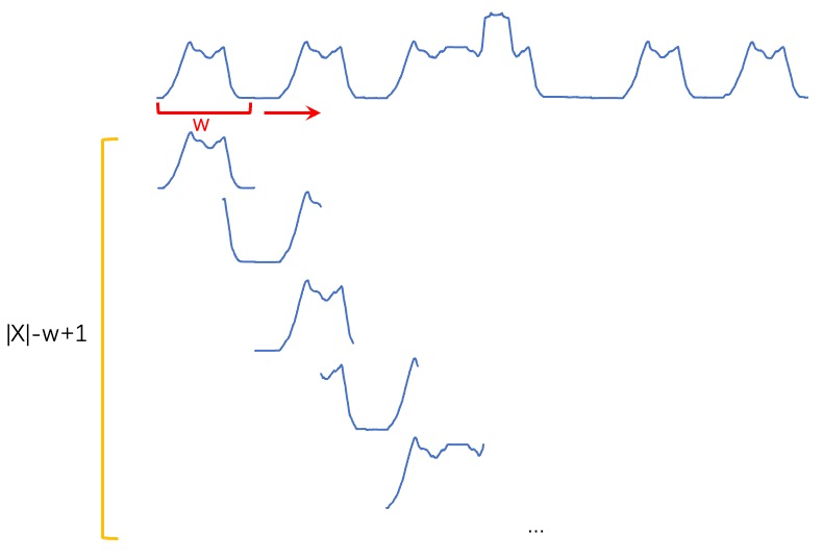
\includegraphics[width=0.66\linewidth]{sliding_window.png}
  \caption{滑动窗口时间序列分段示例}
  \label{fig:sliding_window}
\end{figure}

在滑动窗口模型中,可以直接使用3.1节所述的全局对称性度量算法计算每段时间子序列
的对称性,由于单个时间序列对称性计算的时间复杂度为$O(w^2 )$,所以全部
分段时间序列对称性度量算法的时间复杂度为$O\left(|X| \times w^{2}\right)$。
然而,利用滑动窗口和区间动态规划算法的特点可以将复杂度降低一个阶数。
考虑时间序列$X$两段长度为$w$的连续子序列$S_{i}=\left(\left(t_{i}, x_{i}\right),\left(t_{i+1}, x_{i+1}\right), \dots,\left(t_{i+w-1}, x_{i+w-1}\right)\right)$
和$S_{i+1}=\left(\left(t_{i+1}, x_{i+1}\right),\left(t_{i+2}, x_{i+2}\right), \dots,\left(t_{i+w}, x_{i+w}\right)\right)$的对称度度量,
根据式~\ref{eq:dp_item}的状态方程,时间子序列$S_i$的对称度
$D P(i, i+w-1)$由$DP(i,i+w-2)$,$DP(i+1,i+w-1)$和$DP(i+1,i+w-2)$
的最小值推导而来,而子序列$S_{i+1}$的对称度$D P(i+1, i+w)$由
$D P(i+1, i+w-1)$,$DP(i+2,i+w)$和$DP(i+2,i+w-1)$的最小值推导
而来,这两个对称度的计算都使用到了状态$DP(i+1,i+w-1)$,如果分别计算
将会产生大量的重复计算。然而,考虑到动态规划方程的无后效性,如果先计算
出时间序列$X$中所有长度为$w-1$和$w-2$的子序列对称度并保存下来,
则$S_i$和$S_{i+1}$的状态可以直接计算得到。
图~\ref{fig:fregment}展示了分段时间序列对称度推导过程,
假设时间序列$X$的长度为9,子序列长度即滑动窗口长度为5,采用窗口长度由小到大的
自底向上的推导顺序,每段子序列对称度状态都可以通过$O(1)$的复杂度计算得到,最终所有时间子序列
对称度度量的复杂度由状态个数决定,最底层长度为1的状态有$|X|$个,最顶层
长度为$w$的状态有$|X|-w+1$个,根据等差数列求和共有
$2 \times|X| \times w-w^{2}+w$个状态。
因此,分段时间序列对称度度量算法的渐进时间复杂度为$O(|X| \times w)$,
比通过原始和反转时间序列DTW距离度量对称度的$O\left(|X| \times w^{2}\right)$
效率高一个阶数。
\begin{figure}
  \centering
  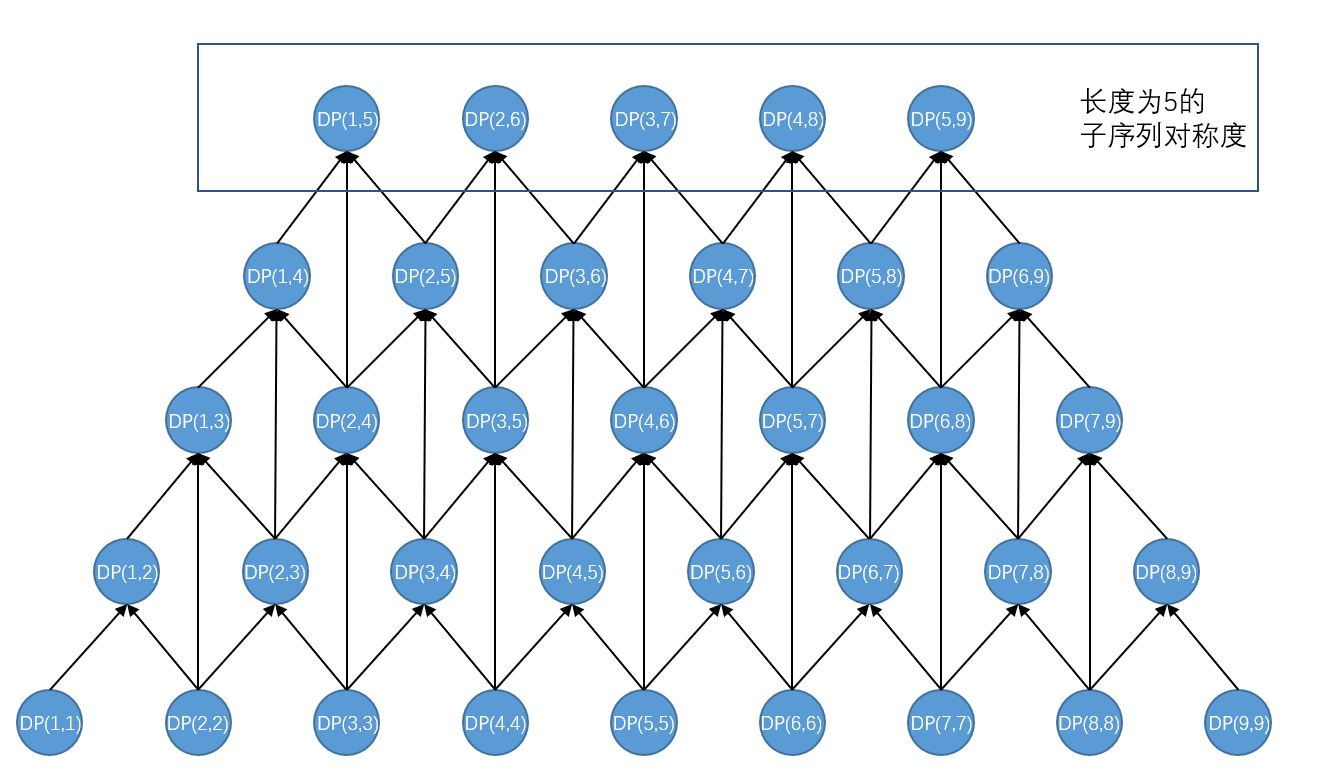
\includegraphics[width=0.76\linewidth]{fregment.png}
  \caption{分段时间序列推导流程}
  \label{fig:fregment}
\end{figure}

\section{分段对称度阈值确定算法}

4.1节讲述了分段时间序列的对称性度量算法,根据4.1节的算法,
给定时间序列X和子序列的长度约束$w$,可以在$O(|X| \times w)$的时间内
计算出所有的子序列对称度。然而,如果想判别出真正的对称时间子序列,
还需要至关重要的一步——确定分段对称度阈值。
图~\ref{fig:lontitude_symmetry}展示了运输车经度标准化处理后的时间序列和对应的分段对称度变化情况。
一般工业场景中,对称度阈值往往是由领域专家输入的。但是,并非所有的
应用场景中都能找到专业的领域专家。并且,如果对称度阈值提供的不合适,
将极大的影响对称模式的挖掘。因此,本节提出了一个基于时间序列数据特征
和对称度分布特征的对称度阈值计算方法。
\begin{figure}
  \centering
  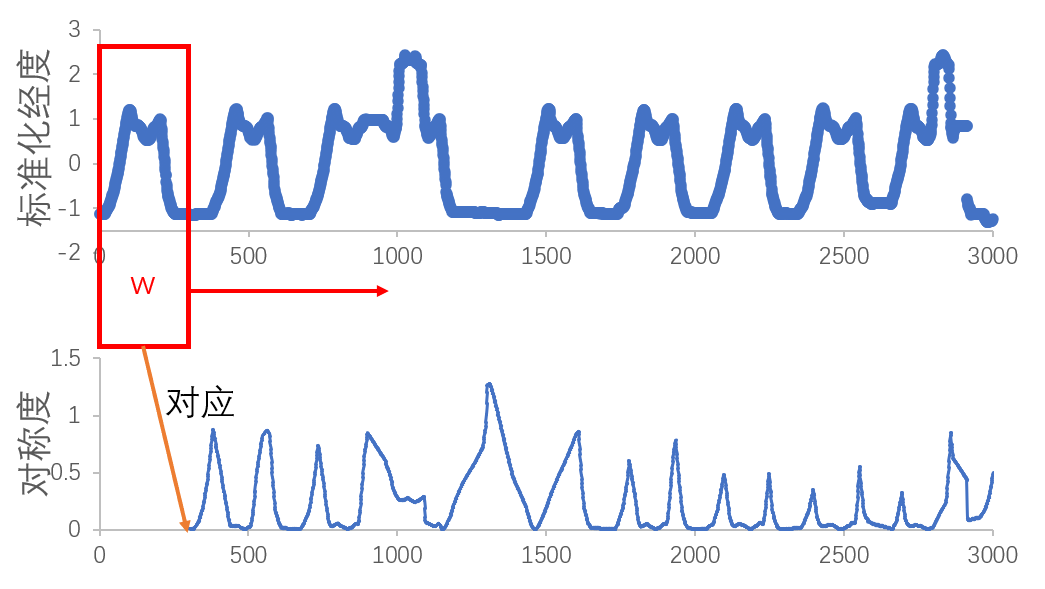
\includegraphics[width=0.76\linewidth]{std_lo_symmetry.png}
  \caption{标准化经度分段对称度变化}
  \label{fig:lontitude_symmetry}
\end{figure}

分段对称度阈值是对所有的时间子序列度量对称性,
因此,除了全局对称度阈值
考虑到的时间序列数据特征,对称度自然分布同样产生阈值划分。
基于时间序列数据特征的阈值确定算法已在3.1.2节中详述,本节只
讨论基于分布特征的对称度阈值确定算法,即$\theta_2$。

在同一类时间序列中,长度相同的对称子序列的对称度较小,
而非对称子序列的对称度较大,这之间存在一个天然的阈值划分。
根据聚类方法\cite{DBLP:conf/kdd/EsterKSX96}和
自然断点分类的划分原则\cite{DBLP:journals/pami/Cheng95},
同一个类簇中数据的相似度高而不同类簇中数据的相似度低。
换言之,两个对称子序列的对称度差距应尽可能小,
而对称子序列与非对称子序列的对称度差距应尽可能大。
在概率统计中,方差用于衡量数据集中数据的偏离程度。
因此,很多算法使用方差作为度量指标变化的阈值\cite{DBLP:conf/sigmod/SongZW16}。
公式~\ref{eq:threshold2}展示了基于方差度量的对称度阈值确定原则,
其中,$DP_i$和$DP_j$均表示计算得到的子序列对称度,$\overline{DP_{i}}$̅和$\overline{DP_{j}}$
表示二者的均值。公式的最优化目标为在子序列对称度组成的集合中,
通过选择某个合适的值作为对称阈值,对称度小于该阈值的子序列为
对称子序列集合,对称度大于该阈值的子序列为非对称子序列集合,
使得对称子序列集合和非对称子序列集合的对称度方差之和最小。
图~\ref{fig:natural_break}展示了在运输车子序列对称度和挖掘机工况子序列对称度中
选择合适的自然断点,可使得对称模式和非对称模式的均值适中,
方差之和最小。综合时间序列数据特征和对称度分布的两类对称度阈值,
最终可以得到对称度阈值的完整公式,即式~\ref{eq:threshold}所示。
\begin{equation}
  \theta_{2}=\underset{x \in D P}{\operatorname{argmin}}\left(\sum_{D P_{i} \leq x}\left(D P_{i}-\overline{D P_{l}}\right)^{2}+\sum_{D P_{j}>x}\left(D P_{j}-\overline{D P_{j}}\right)^{2}\right)
  \label{eq:threshold2}
\end{equation}
\begin{equation}
  \theta=\min \left(\theta_{1}, \theta_{2}\right)
  \label{eq:threshold}
\end{equation}
\begin{figure}
  \centering
  \subcaptionbox{运煤车轨迹子序列对称度\label{fig:natural_break-a}}
  {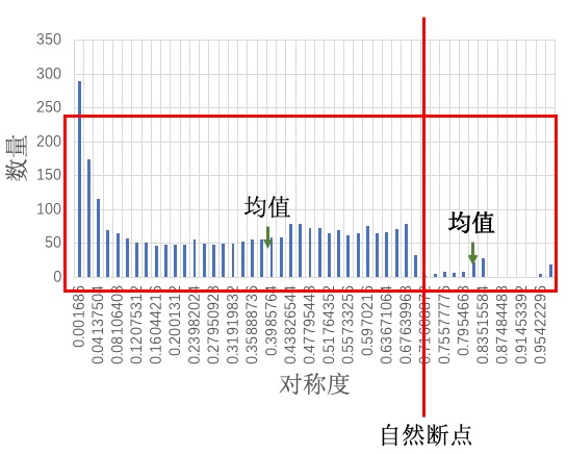
\includegraphics[width=0.42\linewidth]{natural_break-a.png}}
  \subcaptionbox{挖掘机工况子序列对称度\label{fig:natural_break-b}}
  {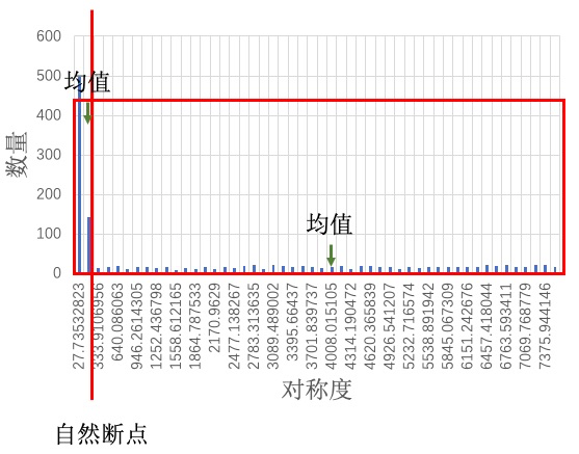
\includegraphics[width=0.42\linewidth]{natural_break-b.png}}
  \caption{运输车轨迹和挖掘机工况子序列对称度分布}
  \label{fig:natural_break}
\end{figure}

\renewcommand{\algorithmicrequire}{\textbf{输入:}\unskip}
\renewcommand{\algorithmicensure}{\textbf{输出:}\unskip}

\begin{algorithm}[t]
  \caption{分段对称度阈值确定算法$calculate\_segment\_threshold$}
  \label{alg:threshold}
  \small
  \begin{algorithmic}
    \REQUIRE 子序列对称度列表$y$,时间序列$X=\left(p_{1}, p_{2}, \dots, p_{n}\right)$
    \ENSURE 分段对称度阈值$\theta$

    \STATE sort$(y)$
    \STATE $a_1 \leftarrow y_1$
    \STATE $i \leftarrow 2$
    \WHILE{$i \leq \left|y\right|$}
    \STATE $a_i \leftarrow a_{i-1}+\frac{y_i-a_{i-1}}{i}$
    \STATE $l_i \leftarrow \frac{i-1}{i \times i} \times(y_i-a_{i-1})^{2}+\frac{i-1}{i} \times l_{i-1}$
    \STATE $i \leftarrow i+1$
    \ENDWHILE

    \STATE reverse$(y)$
    \STATE $a_1 \leftarrow y_1$
    \STATE $i \leftarrow 2$
    \WHILE{$i \leq \left|y\right|$}
    \STATE $a_i \leftarrow a_{i-1}+\frac{y_i-a_{i-1}}{i}$
    \STATE $r_i \leftarrow \frac{i-1}{i \times i} \times (y_i-a_{i-1})^{2}+\frac{i-1}{i} \times r_{i-1}$
    \STATE $i \leftarrow i+1$
    \ENDWHILE

    \STATE reverse$(r)$
    \STATE reverse$(y)$
    \STATE $d \leftarrow l_1 + r_2$
    \STATE $idx \leftarrow 1$
    \STATE $i \leftarrow 2$
    \WHILE{$i < \left|X\right|$}
    \IF{$l_i + r_{i+1} < d$}
    \STATE $d \leftarrow l_i + r_{i+1}$
    \STATE $idx \leftarrow i$
    \ENDIF
    \STATE $i \leftarrow i+1$
    \ENDWHILE
    \STATE $i \leftarrow 1$
    \WHILE{$i < \left|X\right|$}
    \STATE minus $\leftarrow$ minus $+D\left(p_{i}, p_{i+1}\right)$
    \STATE $i \leftarrow i+1$
    \ENDWHILE
    \STATE $\theta \leftarrow \min \left(\frac{minus}{n-1}, \frac{dp_{idx}}{n}\right)$
    \RETURN $\theta$
  \end{algorithmic}
\end{algorithm}

算法~\ref{alg:threshold}给出了分段对称度阈值的计算方法,考虑到
基于对称度分布的阈值确定算法需要用到
动态集合方差的计算,本文采用了流式的方差计算方法。
第1行按照大小顺序对对称度进行排序,为方差的流式计算做准备。
第2-8行根据流式算法计算前i小的对称度方差并保存到数组$l$中,从而得到
顺序排序的前缀方差数组。
第9-16行将对称度倒序排序后计算前$i$大的对称度方差并保存到数组$r$中,
由此得到倒序排序的前缀方差数组。
第17-28行通过计算前$i$小和后$n-i$大的对称度方差之和的最小值
得到基于对称度分布的阈值。
第24-35行计算时间序列相邻点距离的均值得到全局对称度阈值,
并通过和对称度分布阈值比较得到较小者,作为最终的对称度阈值。
采用这种算法得到的对称度阈值不仅考虑到了时间序列本身的特征,
还考虑到了对称度的分布,在实验结果中有良好的表现。

\section{挖掘分段对称模式}

计算出时间序列$X$所有在长度约束范围之内的子序列对称度之后,
可以利用贪心算法挖掘得到所有满足对称性的子序列。以斗杆外摆为例,
在挖掘过程中,存在对称子序列相互包含的情况。如图~\ref{fig:overlap}
中所示,子序列$a$、$b$、$c$均是对称子序列。由于要挖掘不重叠对称子序列,
若结果集合中选择了$a$,则不能再选择$b$和$c$。因此,
为了充分利用时间序列的信息,本文以对称子序列的数量最大值为
优化目标。根据贪心算法的思想,若上一个选择的对称子序列为$s_i$
其长度为$w$,则下一个对称子序列的贪心策略为从数据点$i+w$
开始,选择第1个长度为$w$的对称子序列, 可以保证能得到数量最多的
不重叠子序列。换言之,对于两个长度为$w$且存在重叠的时间序列,选择开始点最早的
时间序列能保证挖掘到数量最多的对称子序列。具体证明如下:假设存在3个长度为$w$的对称子序列
$A=\left(p_{i}, p_{i+1}, \dots, p_{i+w-1}\right)$,$B=\left(p_{j}, p_{j+1}, \dots, p_{j+w-1}\right)$和
$C=\left(p_{k}, p_{k+1}, \dots, p_{k+w-1}\right)$,并且$i<j<k$。若选择A序列进入
对称模式集合,则剩余对称模式可以从$p_{i+w}$之后的点进行选取。若选择B序列进入
对称模式集合,则剩余对称模式可以从$p_{j+w}$之后的点进行选取。由$i<j$可知,
$i+w<j+w$,前者的选择范围比后者更广,如果在选择B序列进入对称模式集合之后仍可选择C序列,
证明$j+w \leq k$,则$i+w$也$\leq k$,同样也可以选择A序列来替换B序列进入对称模式集合。
反之,如果选择A序列进入对称模式集合,则不一定可以由B序列替换。因此,对于长度相同的对称子序列,
选择起始时间点最早的序列能保证挖掘出最多的对称模式。

\begin{figure}
  \centering
  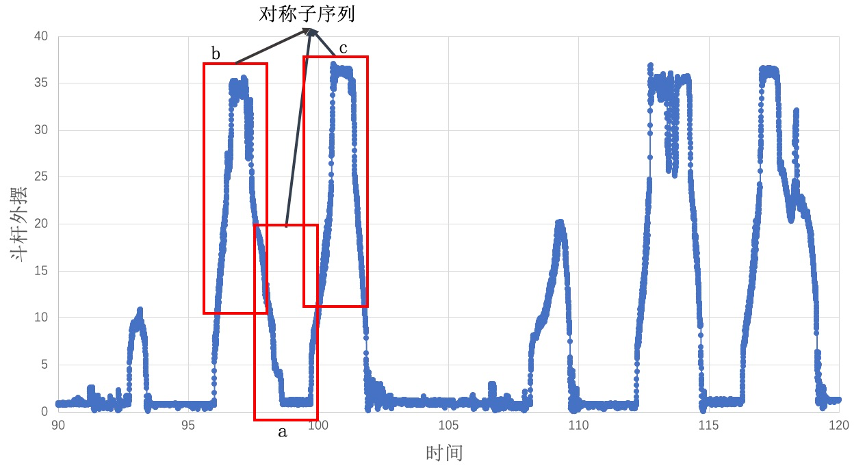
\includegraphics[width=0.80\linewidth]{symmetric_overlap.png}
  \caption{对称时间序列反映重叠现象的案例}
  \label{fig:overlap}
\end{figure}

在运输车轨迹和挖掘机作业等需要挖掘分段对称模式的
实际工业场景中,用户并不关心也没有必要得知所有对称模式的
时间范围,用户关心的只是通过分段对称模式的个数以分析操作人员做功
的数量。因此,本文根据上述分段对称模式挖掘方法提出了相应的具体算法,
以完整的时间序列$X$和子序列长度约束$w$为输入,以对称模式数量为输出,
如算法~\ref{alg:symmetric_pattern}所示。第1-19行根据第3.2节提出的对称度计算方式
计算了给定时间长度约束下所有子序列的对称度,第20行根据算法~\ref{alg:threshold}的计算方式
确定了对称度阈值,第21-30行根据贪心策略
计算出数量最多的不重叠对称子序列。由前述定义可知,第1-19行计算子序列对称度的时间复杂度为$O(|X| \times w)$,
第20行自然断点的确定和不重叠对称子序列的挖掘均只需要$O(|X|)$的时间。
因此,本算法的整体时间复杂度为$O(|X| \times w)$,其效率远远高于直接利用
DTW 计算的$O\left(|X| \times w^{2}\right)$,为后续的数据分析提供数据基础。
\renewcommand{\algorithmicrequire}{\textbf{输入:}\unskip}
\renewcommand{\algorithmicensure}{\textbf{输出:}\unskip}

\begin{algorithm}[t]
  \caption{分段对称模式挖掘算法$calculate\_segment\_symmtric\_pattern$}
  \label{alg:symmetric_pattern}
  \small
  \begin{algorithmic}
    \REQUIRE 时间序列$X=\left(p_{1}, p_{2}, \dots, p_{n}\right)$,长度约束$w$
    \ENSURE 分段对称模式的数量$N$

    \STATE $i \leftarrow 1$
    \WHILE{$i \leq \left|X\right|$}
    \STATE $dp_{i,i} \leftarrow inf$
    \ENDWHILE

    \STATE $i \leftarrow 1$
    \WHILE{$i < \left|X\right|$}
    \STATE $dp_{i,i+1} \leftarrow D\left(p_{i}, p_{i+1}\right)$
    \ENDWHILE

    \STATE $len \leftarrow 3$
    \WHILE{$len \leq \left|X\right|$}
    \STATE $i \leftarrow len$
    \WHILE{$i \leq \left|X\right|-len+1$}
    \STATE $dp_{i,i+len-1} = D\left(p_{i}, p_{i+1}\right)+\min \left(dp_{i,i+len-2},dp_{i+1,i+len-1},dp_{i+1,i+len-2}\right)$
    \ENDWHILE
    \ENDWHILE

    \STATE $i \leftarrow 1$
    \WHILE{$i \leq \left|X\right|-w+1$}
    \STATE $y_i=dp_{i,i+w-1}$
    \ENDWHILE
    \STATE $\theta = calculate\_threshold\left(y,X\right)$

    \STATE $i \leftarrow 1$
    \WHILE{$i \leq \left|X\right|-w+1$}
    \IF{$dp_{i,i+w-1}/w \leq \theta$}
    \STATE $N \leftarrow N + 1$
    \STATE $i \leftarrow i+w$
    \ELSE
    \STATE $i \leftarrow i+1$
    \ENDIF
    \ENDWHILE
    \RETURN $N$
  \end{algorithmic}
\end{algorithm}

\section{基于IoTDB的分段对称模式挖掘算法设计}

Apache IoTDB是面向时间序列的原生数据库,是一个集
数据收集、存储和分析于一体的数据管理引擎,不仅提供了类SQL
的数据查询功能,而且预留了基于元数据和UDF(User Defined 
Function)接口的数据分析功能,具有高度的可扩展性。本节将利用
IoTDB提供的数据分析接口设计并优化分段对称模式挖掘算法。

在IoTDB提供的分析功能两种扩展方式中,基于UDF的方式较为简单。
通过实现系统设计的自定义时间序列生成函数(UDTF)接口,用户根据
自定义的数据获取策略得到固定长度且已经对齐的
单条或多条时间序列分段,之后便可以在这些分段数据上编写分析函数
逻辑,得到结果后以时间序列的方式输出到结果集中。这种方式的好处
有二,一是实现简单,不需要考虑底层存储和上层查询解析,只需要
对已处理好的数据进行分析。二是其实现不会对任何写入负载产生影响,
基于UDF的数据分析功能不需要在写入时保存信息,在查询的过程中
执行分析计算,适合读少写多的用户场景。尽管如此,基于UDF方式的缺点
也十分明显,其所有的计算都在查询过程中计算,大大增加了查询的时间损耗,
而且查询结果是一次性的,后发查询并不会因为前发查询计算过相同
时间内的数据就会优化计算。对于分段对称模式挖掘算法而言,
一次查询的时间复杂度为$O(|X| \times w)$,当时间序列长度过高
或者窗口长度过大时,一次查询计算的时间损耗将变得难以忍受。因此,
本节主要考虑基于IoTDB数据库的元信息对分段对称模式挖掘算法进行性能优化。

为了加快IoTDB原生聚合分析查询的效率,IoTDB在用户执行数据写入操作时,
会保存若干类元信息。这涉及到了IoTDB的底层数据存储文件TsFile的内容。
如图~\ref{fig:iotdb}所示,Tsfile包含3个层级的存储单元,由大到小
分别是ChunkGroup数据块组,Chunk数据块和Page数据页。
伴随着时间序列数据的写入,在Chunk数据块和Page数据页之间会存储
相关的元数据信息,分别存储在ChunkHeader和PageHeader结构中。
其中,ChunkHeader主要存储传感器名称、数据大小、数据和压缩类型以及
page数量等等,而PageHeader中却会存储包括数据点个数,开始与结束时间,
最大最小值,首值尾值,数据和以及极值等关键统计信息。
这些Page上的元信息在内置聚合函数上取得了显著的加速效果,
在千万以上的数据量下仍然能够在几十毫秒时间内完成查询
\cite{DBLP:conf/cikm/Huang0WZW16}。
因此,如果在PageHeader中增加关于分段对称模式挖掘的元信息,
尽管在数据写入阶段会使得性能略有降低,但却极大地提高了查询时
模式挖掘的时间效率,并且持久化的元信息支持多次查询,一写多读
的方式对于分段对称模式挖掘这种查询分析效率较低为性能瓶颈的
操作具有重大意义。因此,本节利用IoTDB的元数据特性,
通过调整和优化分段对称模式挖掘算法,使其时间性能大幅提升。
\begin{figure}
  \centering
  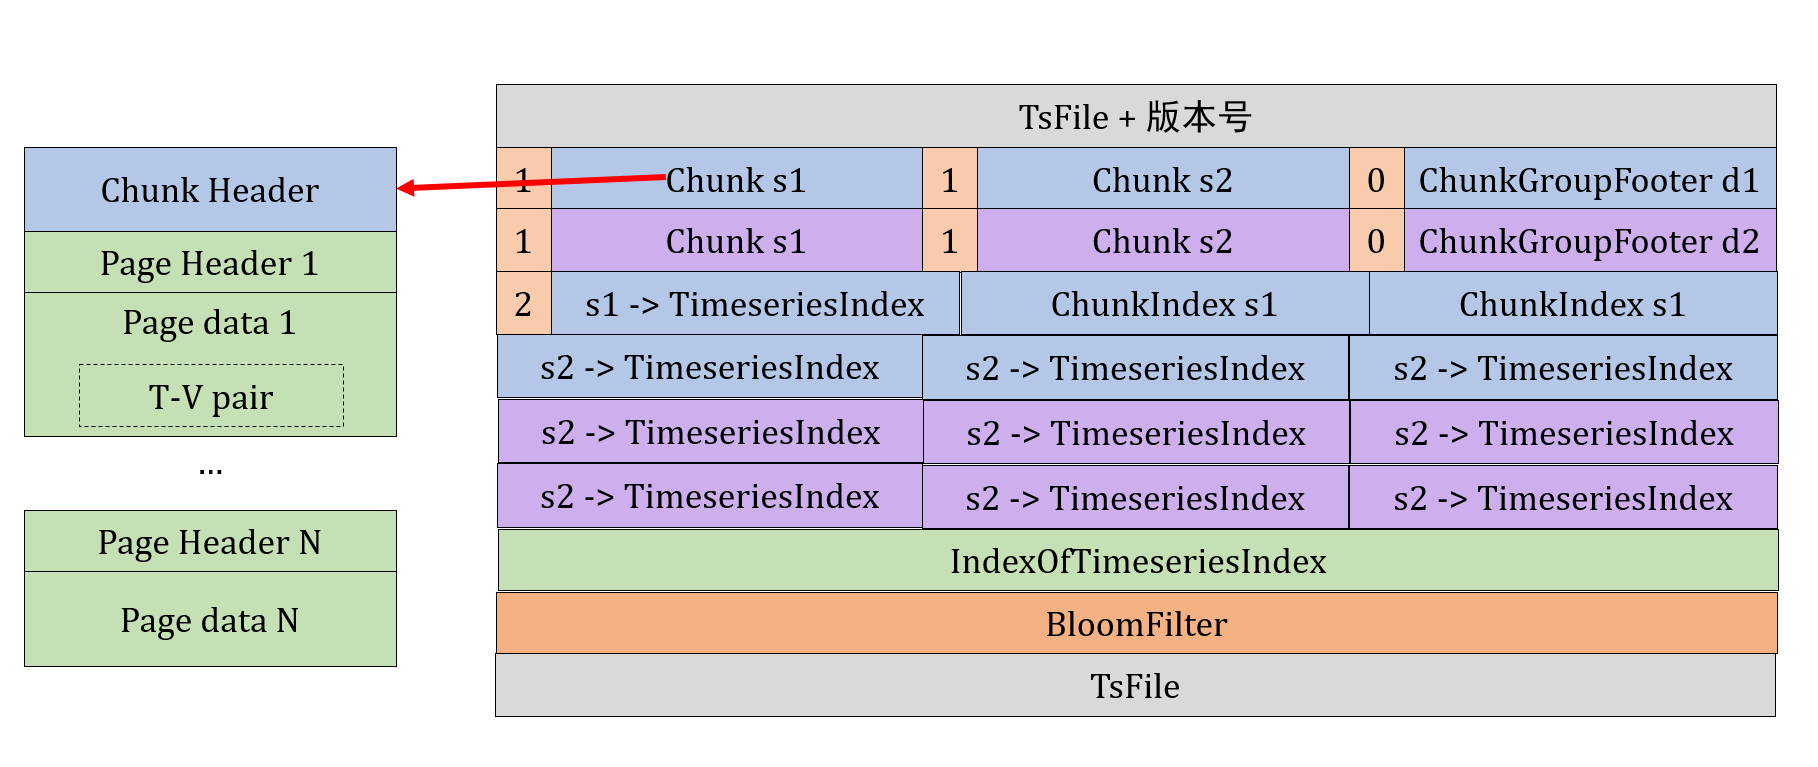
\includegraphics[width=1.0\linewidth]{IoTDB_data_storage.png}
  \caption{IoTDB底层存储和元数据信息}
  \label{fig:iotdb}
\end{figure}

将分段对称模式挖掘算法应用于IoTDB首先需要解决的一个问题
就是时间序列在多个Page存储时,如何在merge计算时
挖掘出跨多个Page的对称模式。在PageHeader的元信息中
根据子序列长度约束$w$保存前一个Page末尾长度为$w$的时间序列原始点
是保证对称模式挖掘完整性最暴力的方式。这种方式可以保证
基于元数据的分段对称模式挖掘结果和基于UDF的挖掘结果完全一致。
但是,当$w$太大时,这种暴力方式却需要在PageHeader的元信息中
保存过多的数据,增加了序列化和反序列化的时间开销,也浪费了
宝贵的存储空间。考虑蕴含分段对称模式的时间序列的数据特征,
不管时间序列包含了多少个分段对称模式,根据第2章中的定义,
其必然是互不重叠的。因此,可以根据分段对称模式的物理断点确定
IoTDB存储Page的点数上限,保证不存在跨Page的分段对称模式。
这样就不需要在元信息中存储过多的原始点信息。
接下来主要介绍
如何根据IoTDB的写入流程具体优化分段对称模式挖掘算法。


\subsection{单点更新内存状态}

如上所述,Page的元数据存储结构PageHeader既然能存储最值,总和等信息,
那自然也能存储分段对称模式相关的元数据。考虑IoTDB的数据写入流程,
由于IoTDB的存储引擎是基于LSM\cite{DBLP:journals/vldb/LuoC20}设计的,其写入步骤分为两步,
首先先写入到内存缓冲区memtable中,当Page写满时将内存数据刷写到磁盘。
在这个过程中,写入到memtable是实时写入,
而memtable的刷写则是通过后台线程并发执行。
因此,分段对称模式挖掘算法需要尽量降低每次写入的时间复杂度。
这需要分两步考虑算法的性能优化。首先是在写入到memtable的阶段,
在每个新数据点插入到IoTDB中时,时间序列可以认为是流式数据,
通过对3.4.1节的流式时间序列对称性度量算法进行扩展和优化,
可以很方便的将全局算法推演到分段算法。只需要在每个数据点$p_t$
来时利用流式算法在$O(w)$的时间内按照倒序的时间顺序
计算出从点$p_{t-1}$,$p_{t-2}$到$p_{t-w+1}$与$p_t$范围内
时间子序列的对称度,并保存在流式计算状态中即可。
为了节省空间,分段对称模式流式挖掘通过维护一个循环使用的
长度为$w$的对称度列表$dp$,用于保存与点$p_t$相关的单列对称度状态。
此外,需要同步保存的状态包括一个Page内分段时间序列的对称度列表$sym$
和与$p_t$在同一个窗口$w$内的流式时间序列$X$。这些状态都只会保存在
内存中,并不会即时刷写到磁盘存储的元数据中。

\renewcommand{\algorithmicrequire}{\textbf{输入:}\unskip}
\renewcommand{\algorithmicensure}{\textbf{输出:}\unskip}

\begin{algorithm}
  \caption{分段对称模式流式状态更新$calculate\_streaming\_status$}
  \label{alg:iotdb_streaming}
  \small
  \begin{algorithmic}
    \REQUIRE 新数据点$p_t$,长度约束$w$
    \ENSURE 流式时间序列$X$,流式分段对称度列表$sym$,流式对称度状态$dp$

    \IF{$t = 1$}
        \STATE $dp_{1} \leftarrow 0$
    \ELSE
      \STATE $\theta_1 \leftarrow \theta_1 + D\left(p_{t}, p_{t-1}\right)$
      \STATE $dp_1^{\prime} \leftarrow 0$
      \STATE $ idx \leftarrow 1$
      \WHILE{$ idx \leq |dp|$}
        \STATE $ idx \leftarrow idx+1$
        \IF{$idx = 2$}
          \STATE $dp_{idx}^{\prime} \leftarrow D\left(p_{t}, p_{t-idx-1}\right)$
        \ELSE
          \STATE $dp_{idx}^{\prime} \leftarrow D\left(p_{t}, p_{t-idx-1}\right)+min(dp_{idx},dp_{idx-1},dp_{idx-1}^{\prime})$
        \ENDIF
      \ENDWHILE
      \STATE $ dp \leftarrow dp^{\prime}$
      \IF{$|dp| = w$}
        \STATE $sym_{t-w+1} \leftarrow dp_{w}$
        \STATE 删除$dp$的队首元素
      \ENDIF
    \ENDIF
    \STATE 将$p_t$置于流式时间序列$X$中
    \IF{$|X| = w$}
      \STATE 删除$X$的队首元素
    \ENDIF
  \end{algorithmic}
\end{algorithm}

具体的计算流程如算法~\ref{alg:iotdb_streaming}所示,其中,第1-3
行初始化流式对称度状态$dp$,第4-15行对与$p_t$在同一个窗口的对称度
状态进行流式更新,第16-20行将长度为$w$的子序列对称度保存到$sym$中,
第20-24行把$p_t$点置入流式时间序列$X$并删除无效点。
由算法可知,经过分段对称模式挖掘流程的分解,单点写入memtable
只需要$O(w)$时间复杂度之内的流式状态更新,而$w$的值一般设置较小,
故其对写入负载的影响较小。

\subsection{合并计算分段对称模式元数据}

接下来需要考虑如何在memtable的刷写阶段挖掘出分段对称模式。
在通过流式算法计算出分段时间序列的对称度之后,再计算出分段对称度
阈值就可以挖掘出分段对称模式。为简化计算,本节用单个Page内
的分段对称度阈值挖掘同一个Page内的分段对称模式。
而分段对称度阈值$\theta$由基于时间序列数据特征的阈值$\theta_1$
和基于对称度分布的阈值$\theta_2$共同决定。
对于$\theta_1$,只需要在
在写入到memtable的阶段与保存的前置点状态进行差分即可计算。
至于$\theta_2$,则需要在memtable刷写阶段根据保存好的时间子序列
对称度集合以非对称模式对称度和对称模式对称度方差之和为优化目标,
计算出子序列对称度的自然断点。通过$\theta_1$和
$\theta_2$的最小值即可得到对称度阈值$\theta$,由其过滤即可得到
对称模式,将其数量信息保存在PageHeader的元数据中。
具体计算流程如算法~\ref{alg:iotdb_streaming_flush}所示,
第1-2行计算得到分段对称度阈值,第3-12行通过阈值过滤对称度列表
得到分段对称模式的数量信息。
由于需要遍历全部分段对称度列表$sym$,故其时间复杂度为$O(n)$,
但由于memtable刷写到磁盘的操作是在后台线程并发执行的,并不会过分影响性能。

\renewcommand{\algorithmicrequire}{\textbf{输入:}\unskip}
\renewcommand{\algorithmicensure}{\textbf{输出:}\unskip}

\begin{algorithm}
  \caption{分段对称模式元数据计算$calculate\_segment\_metadata$}
  \label{alg:iotdb_streaming_flush}
  \small
  \begin{algorithmic}
    \REQUIRE 最后一个数据点$p_n$,长度约束$w$,流式分段对称度列表$sym$
    \ENSURE 分段对称模式数量$N$
    \STATE 计算sym流式分段对称度列表的自然断点$\theta_2$
    \STATE $\theta \leftarrow min(\frac{\theta_1}{n-1},\theta_2)$

    \STATE $i \leftarrow 1$
    \WHILE{$i \leq \left|sym\right|$}
    \IF{$\frac{sym_{i}}{w} \leq \theta$}
    \STATE $N \leftarrow N+1$
    \STATE $i \leftarrow i+w$
    \ELSE
    \STATE $i \leftarrow i+1$
    \ENDIF
    \ENDWHILE
    \RETURN $N$
  \end{algorithmic}
\end{algorithm}

综上,本节根据IoTDB的存储和计算方式优化了分段对称模式挖掘算法。
IoTDB的底层存储文件TsFile中预留了可用于加速查询分析的元数据信息,
通过将分段对称模式挖掘算法产生的中间结果保存到元数据中,
可以大大提高查询计算的时间效率。而且,经过优化,
分段对称模式挖掘算法分为了流式状态更新和元数据更新。其中,
单点写入的流式状态更新的操作复杂度仅为$O(w)$,只与子序列长度约束有关。
而元数据更新的操作复杂度虽然为$O(n)$,但其是在后台线程并发执行,
并不会过分影响写入性能。因此,基于元数据的分段对称模式挖掘算法很好的
平衡了查询和写入时间效率。在第5章的实验中,本文比较了基于UDF和元数据
的分段对称模式挖掘效率,证明了基于元数据的算法在实际应用中的有效性。


\section{本章小结}
本章主要介绍了分段时间序列对称模式挖掘的算法框架和优化扩展。
首先根据对称子序列长度约束$w$,定义了基于全局最优匹配和区间动态规划
算法思想的分段时间序列对称性度量算法。然后,
在3.2节根据时间序列的数据特征和对称度的分布特征提出了
分段对称度阈值的确定算法
并在3.3节利用贪心策略和分段对称度阈值过滤得到了分段对称模式。
最后,本文根据Apache IoTDB的存储和计算方式
对分段对称模式挖掘算法进行了优化。
根据第5章的实验证明,本节所定义的分段对称模式挖掘算法
在不同来源的数据集上具有更高的准确性和鲁棒性,
而且其效率比基于动态时间扭曲的算法
高出了一个阶数。此外,通过在IoTDB系统中
对比基于UDF和元数据的分段对称模式挖掘算法的性能,
发现基于元数据的方法对计算查询的效率提升明显。
% 模板支持 BibTeX 和 BibLaTeX 两种方式处理参考文献。
% 下文主要介绍 BibTeX 配合 \pkg{natbib} 宏包的主要使用方法。


% \section{顺序编码制}

% 在顺序编码制下,默认的 \cs{cite} 命令同 \cs{citep} 一样,序号置于方括号中,
% 引文页码会放在括号外。
% 统一处引用的连续序号会自动用短横线连接。

% \thusetup{
%   cite-style = super,
% }
% \begin{tabular}{l@{\quad$\Rightarrow$\quad}l}
%   \verb|\cite{zhangkun1994}|               & \cite{zhangkun1994}               \\
%   \verb|\citet{zhangkun1994}|              & \citet{zhangkun1994}              \\
%   \verb|\citep{zhangkun1994}|              & \citep{zhangkun1994}              \\
%   \verb|\cite[42]{zhangkun1994}|           & \cite[42]{zhangkun1994}           \\
%   \verb|\cite{zhangkun1994,zhukezhen1973}| & \cite{zhangkun1994,zhukezhen1973} \\
% \end{tabular}


% 也可以取消上标格式,将数字序号作为文字的一部分。
% 建议全文统一使用相同的格式。

% \thusetup{
%   cite-style = inline,
% }
% \begin{tabular}{l@{\quad$\Rightarrow$\quad}l}
%   \verb|\cite{zhangkun1994}|               & \cite{zhangkun1994}               \\
%   \verb|\citet{zhangkun1994}|              & \citet{zhangkun1994}              \\
%   \verb|\citep{zhangkun1994}|              & \citep{zhangkun1994}              \\
%   \verb|\cite[42]{zhangkun1994}|           & \cite[42]{zhangkun1994}           \\
%   \verb|\cite{zhangkun1994,zhukezhen1973}| & \cite{zhangkun1994,zhukezhen1973} \\
% \end{tabular}



% \section{著者-出版年制}

% 著者-出版年制下的 \cs{cite} 跟 \cs{citet} 一样。

% \thusetup{
%   cite-style = author-year,
% }
% \begin{tabular}{l@{\space$\Rightarrow$\space}l}
%   \verb|\cite{zhangkun1994}|                & \cite{zhangkun1994}                \\
%   \verb|\citet{zhangkun1994}|               & \citet{zhangkun1994}               \\
%   \verb|\citep{zhangkun1994}|               & \citep{zhangkun1994}               \\
%   \verb|\cite[42]{zhangkun1994}|            & \cite[42]{zhangkun1994}            \\
%   \verb|\citep{zhangkun1994,zhukezhen1973}| & \citep{zhangkun1994,zhukezhen1973} \\
% \end{tabular}

% \vskip 2ex
% \thusetup{
%   cite-style = super,
% }
% 注意,引文参考文献的每条都要在正文中标注
% \cite{zhangkun1994,zhukezhen1973,dupont1974bone,zhengkaiqing1987,%
%   jiangxizhou1980,jianduju1994,merkt1995rotational,mellinger1996laser,%
%   bixon1996dynamics,mahui1995,carlson1981two,taylor1983scanning,%
%   taylor1981study,shimizu1983laser,atkinson1982experimental,%
%   kusch1975perturbations,guangxi1993,huosini1989guwu,wangfuzhi1865songlun,%
%   zhaoyaodong1998xinshidai,biaozhunhua2002tushu,chubanzhuanye2004,%
%   who1970factors,peebles2001probability,baishunong1998zhiwu,%
%   weinstein1974pathogenic,hanjiren1985lun,dizhi1936dizhi,%
%   tushuguan1957tushuguanxue,aaas1883science,fugang2000fengsha,%
%   xiaoyu2001chubanye,oclc2000about,scitor2000project%
% }。
